\documentclass{beamer}

\usetheme{Dresden}
\usecolortheme{beaver}

% \usepackage{amsmath}
% \usepackage{amsthm}
\usepackage{graphicx,epstopdf}
\theoremstyle{plain}
\newtheorem{thm}{Theorem}


\title{Pokemon Collector}
\subtitle{First Generation}
\author{Kongsak Tipakornrojanakit}
\institute{Mahidol University, International College}
\date{Dec 2, 2016}
\begin{document}
	
	\begin{frame}
		\titlepage
	\end{frame}
	
	\section{Road to Pokemon Master}
	\begin{frame}
		\frametitle{Table of Contents}
		\tableofcontents[currentsection]
	\end{frame}
	
	\begin{frame}
		\frametitle{There are 151 different Pokemon}
		
		\begin{figure}
			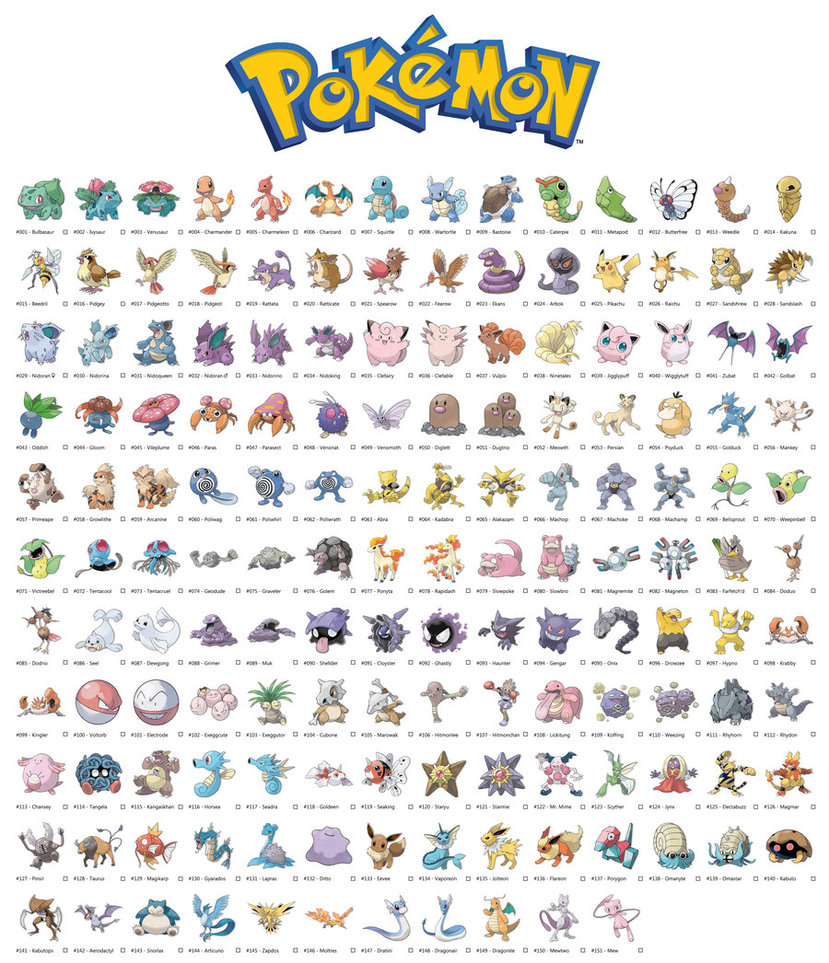
\includegraphics[scale=.8]{Gen1List.jpg}
		\end{figure}
	\end{frame}
	
	
	\section{How many PokeBall do we need ?}
	\begin{frame}
		\frametitle{Table of Contents}
		\tableofcontents[currentsection]
	\end{frame}
	\begin{frame}
		\frametitle{How many PokeBall do we need ?}
		\begin{figure}
			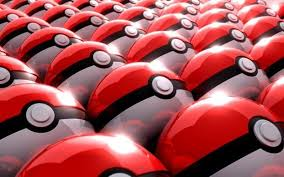
\includegraphics[scale=.8]{pokeball_pile.jpeg}
		\end{figure}		
		
	\end{frame}
	
	
	\begin{frame}
		\frametitle{How many PokeBall do we need ?}
		
		\onslide<1-> There are 151 different Pokemon we need to catch [N = 151] \\ \vspace{10pt}
		
		\onslide<2-> Let $P_k$ be the probability of finding a \textbf{new} k-th Pokemon \\
		\onslide<3-> Let $T_k$ be the number of Pokemon we need to catch before finding the \textbf{new} k-th Pokemon \\
		\onslide<4-> Let $E_k$ be the expected number of Pokemon we need to catch in order to have $k+1$ unique Pokemons \\ \vspace{10pt}
			
		\onslide<5-> Then $P_k$ should be equal to $\frac{N - k}{N}$. \\ \vspace{5pt}
		\onslide<6-> This mean that $T_k$ has geometric distribution with expected value of $\frac{1}{P_k}$ \\ \vspace{5pt} 
		\onslide<7-> Therefore, $E_n = \sum_{k = 0}^{n - 1}{\frac{1}{P_k}}$ 
		
	\end{frame}
	
	\begin{frame}
		\frametitle{How many PokeBall do we need ?}

		\begin{tabular}{l l}
		\onslide<1-> 	$E_n$ 	&$= \sum_{k = 0}^{n - 1}{\frac{1}{P_k}} $ \vspace{10pt} \\ 
		\onslide<2-> 	& $= \sum_{k = 0}^{n - 1}{\frac{n}{n - k}} $		\vspace{10pt} \\  
		\onslide<3-> 	& $= n\,\sum_{k = 0}^{n - 1}{\frac{1}{n - k}} $	\vspace{10pt} \\  
		\onslide<4-> 	& $= n\,\sum_{k = 1}^n{\frac{1}{k}} $	\vspace{10pt} \\
		\onslide<5->	& $= n\,H_n$
		\end{tabular}

	
	\end{frame}

	\section{What if we want 2 of each, or 3 or 4 even ?}
	\begin{frame}
		\frametitle{Table of Contents}
		\tableofcontents[currentsection]
	\end{frame}
	\begin{frame}
		\frametitle{Growth of Average Number of Pokemon to catch to complete n set ?}
		\onslide<2->\begin{figure}
			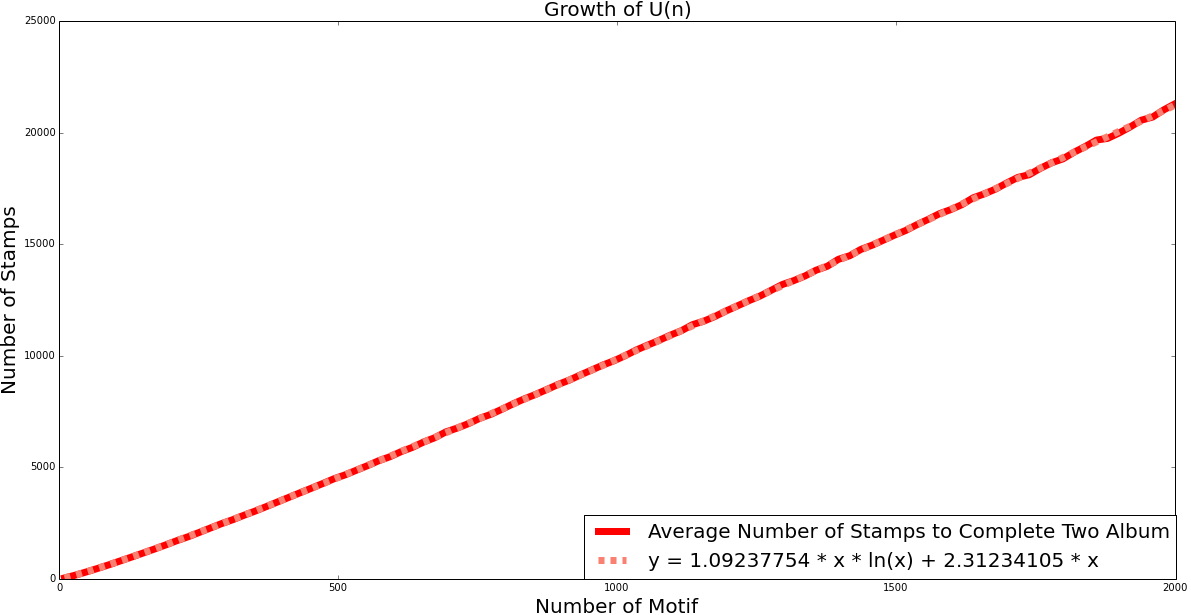
\includegraphics[scale=.25]{Graph.png}
		\end{figure}		
		
	\end{frame}
		
	\section{Questions ?}
	\begin{frame}
		\begin{figure}
			
\includegraphics[scale=.20]{Qman.png}
		\end{figure}
	\end{frame}
	
\end{document} 